 % last updated in April 2002 by Antje Endemann
% Based on CVPR 07 and LNCS, with modifications by DAF, AZ and elle, 2008 and AA, 2010, and CC, 2011; TT, 2014; AAS, 2016

\documentclass[runningheads]{llncs}
\usepackage{graphicx}
\usepackage{amsmath,amssymb} % define this before the line numbering.
\usepackage{ruler}
\usepackage{color}
\usepackage[width=122mm,left=12mm,paperwidth=146mm,height=193mm,top=12mm,paperheight=217mm]{geometry}
\usepackage{appendix}

\begin{document}
% \renewcommand\thelinenumber{\color[rgb]{0.2,0.5,0.8}\normalfont\sffamily\scriptsize\arabic{linenumber}\color[rgb]{0,0,0}}
% \renewcommand\makeLineNumber {\hss\thelinenumber\ \hspace{6mm} \rlap{\hskip\textwidth\ \hspace{6.5mm}\thelinenumber}}
% \linenumbers
\pagestyle{headings}
\mainmatter
\def\ECCV18SubNumber{***}  % Insert your submission number here

\title{Denoising 3D Time-Of-Flight Data} % Replace with your title

\titlerunning{ECCV-19 \ECCV18SubNumber}

\authorrunning{ECCV-19 \ECCV18SubNumber}

\author{Kapil Gupta, Yanwen Xu}
\institute{University of California, Santa Cruz}


\maketitle

\begin{figure}
    \centering
    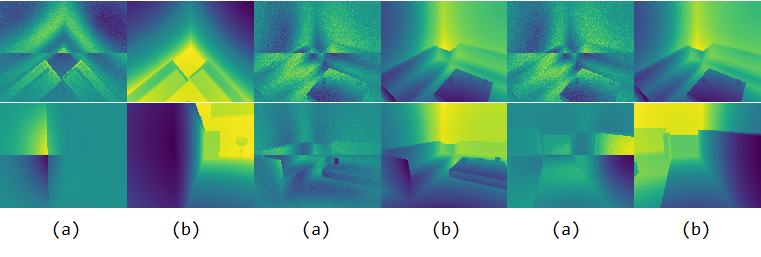
\includegraphics[scale=0.6]{img/depthmap/Figure_1.png}
    \caption{
    From noisy depth images corrupted by Multi-path Interference (left of each pair) to high-accurate depth images (right of each pair), our two-part CNN model can efficiently and robustly remove artifacts in synthesized Time-of-Flight camera images. }
    % Pairs of False Depth Map with MPI Error and True depth map generated by our model.
    \label{fig:result_raw}
\end{figure}

\begin{abstract}
Depth Perception is widely used in several computer vision tasks.
The most common method for depth calculation is range imaging cameras such as Time of Flight (ToF) cameras.  
However, ToF cameras suffer from non-negligible noise caused by Multi-Path Interference (MPI). 
While various classical methods exist, machine learning techniques have not been explored as much due to the lack of ground-truth data. 
In this paper, we propose a novel method for MPI noise removal using a two-part convolutional neural network.  
The first model learns about the core properties of the reflective objects in the scene, such as the reflectively of the scene and local ambient light density.  
The second model learns to map such properties along with a False Depth Map to create a True Depth Map of the scene. 
We demonstrate and validate our results on a synthetic dataset.

\keywords{time-of-flight, multi-path interference, deep learning}
\end{abstract}

% -----------------------------------------------------------------------------------------------------
\section{Introduction}
% -----------------------------------------------------------------------------------------------------

3D imaging systems provide depth information that is crucial in a diverse range of computer vision applications. Depth Sensors using Time-of-Flight(ToF) imaging are the most popular amongst such cameras due to cheap cost. 
Range Imaging and Depth Perception that is available from such cameras can be used for several computer vision tasks such as gesture recognition, image quality improvement, and obstacle avoidance. 
Nevertheless, ToF cameras suffer from various sources of noise caused by the following: the presence of ambient light, the interference due to different modulating frequencies, the noise caused by multiple reflections, the motion introduced by the subject, and the shot noise by the camera's electronics.
In this paper, we focus on the noise caused due to multiple reflections that makes accurate depth calculations difficult. 
\newline
\newline
ToF cameras send a pulsed ray of light and record the time taken for the light ray to reach the sensor. 
The time taken is used to calculate the distance of an object in the scene from the camera. 
The camera's depth map acquisition is based upon the assumption that the ray of light is reflected only once in the given scene before reaching the sensor. 
However, objects with different specularity can scatter light differently, causing multiple reflections with different objects present in the scene. 
The delay caused by multiple reflections causes an error in the depth calculation. 
This is an inherently hard problem because the level of MPI error depends on the properties of objects in the scene, as well as the ambient lighting of the scene.
\newline
\newline
% Talks about previous works
% 
Previous solutions \cite{tomasi1998bilateral,zhang2014rolling} to this issue are performing traditional approaches such as Bilateral filtering on the depth image. 
Bilateral filtering is suitable for Photon Shot Noises because of its nature of taking the average intensity of nearby pixels. 
However, traditional approaches are not necessarily optimal for MPI noises because of its complexity. 
Particularly for MPI denoising, attempts have been made, such as modifying the reflection to get away with errors. 
However, this approach is neither generic nor practical in real-world applications. 
Convolutional Neural Networks (CNN) were commonly used in image denoising. 
Other data-driven approaches \cite{bolsee2018cnn,marco2017deeptof} takes advantage of machine learning, which is to train deep neural networks with synthetic data generated by ToF simulators. 
While the network can somewhat reduce artifacts, it does not entirely remove them. 
Moreover, it still reminds uncertain that if the model trained from synthetic data would apply to real-world data. 
\newline
\newline
We propose a novel method for removing noise caused due to Multi-Path Interference. 
We use a two-part Convolutional Neural Network that is trained on synthetic data. 
The first CNN is used to learn the essential properties of the scene, such as the specularity of objects present in the scene, ambient light, and camera position. 
The second CNN takes the given parameter values from the first model, along with a noisy depth map to generate the true depth map.
Our method is based on the observation that MPI noise is directly dependent upon properties of the scene, and hence learning those properties can help determine the depth map with accurate depth information.
\newline
\newline
We describe our contribution as following: 
\begin{enumerate}
    \item A two-stage training strategy, which first extracts important scene parameters from a noisy depth map and then uses those parameters along with a noisy depth map to create a highly-accurate depth map.  
    \item A practical trained network that removes MPI noise from a single ToF image in real-time and outperforms the state-of-art methods.
    \item A method that is able to process highly specular objects in a scene that may introduce high MPI noise.
\end{enumerate}



% -----------------------------------------------------------------------------------------------------
\section{Related Work}
% -----------------------------------------------------------------------------------------------------

3D cameras send a modulated wave of light that may hit objects in an area and get reflected back with a phase shift in the wave. 
When the reflected wave of light reaches the camera, the phase shift between the original and reflected wave can be used to get the depth value of the object. 
When there is a phase shift in the light received by the camera that was not caused by a single reflection with an object, this causes noise/error in the depth calculation, also called MPI noise.
This noise can occur due to reflective objects in the scene, that disperses light in a way that multiple ways of light intersect with each other. 



% \subsection{Physics-based approaches}

% \subsection{Learning-based approaches}

% Several works was been done using deep learning based approaches, such as CNN and Auto-encoder. 

% In the work \cite{bolsee2018cnn}


\subsection{Classical approaches} MPI Error is caused due to multiple photon intersections, leading to an error in measurements. 
If multiple modulation frequencies of light are used, the time delay operator can be used to process the measurements in the Fourier domain\cite{bhandari2016}. 
In a controlled setting, 2K+1 measurements are needed to recover depth information from K interfering rays of light\cite{bhandari2015}. 
Local and global illumination information has also been used along with the depth information recovered by the ToF camera to overcome MPI based noise\cite{naik2015}.
Light Transport methods that are based on the idea that direct light follows the epipolar line and indirect light does not have been successfully used to remove indirect light from the scene\cite{otoole2014}. 
Further work has been done in separating various transformations indirect light caused by the path of light in the scene in the temporal domain\cite{otoole2014siggraph}
For several other interesting approaches to MPI based noise correction, the reader should refer to the survey paper by Whyte et al. \cite{whyte2014}
.

\subsection{Learning based Methods}
Due to substantial data requirements for this approach, and lack of available datasets with high-quality ground-truth, Deep Learning approach has not been widely used yet. 
Qi et al. used the Transient Rendering method to generate scenes with varying specular properties and ambient lighting conditions. Along with a simulator for introducing noise into the scenes, Qi et al. created a pipeline method \cite{guo2018flat} to correct various noises simulated by the dataset, including shot noise, multi-path inference noise, noise introduced by dynamic scenes.  
A two-network ad-hoc method for depth refinement has been used, where a coarse network first learns the global structure, and then another network attempts to remove MPI noise while preserving details.
GAN\cite{agresti2019unsupervised} was used to perform domain adaptation from synthetic data to real data after learning to remove MPI noise using a CNN based model. A self-supervised method \cite{sterzentsenko2019} that uses deep Auto-encoder along with geometric priors taken from differentiable rendering was also used to remove MPI error. 
\newline
\newline
Even though there have been several papers using synthetic data, the performance on the real dataset has not been that great. 
This is possible because the statistical patterns of noise seen in real-world data cannot be patterned well by the synthetic dataset.

% ========================================================================================
% Data Section
% ========================================================================================

\section{Dataset} 

\begin{figure}
    \centering
    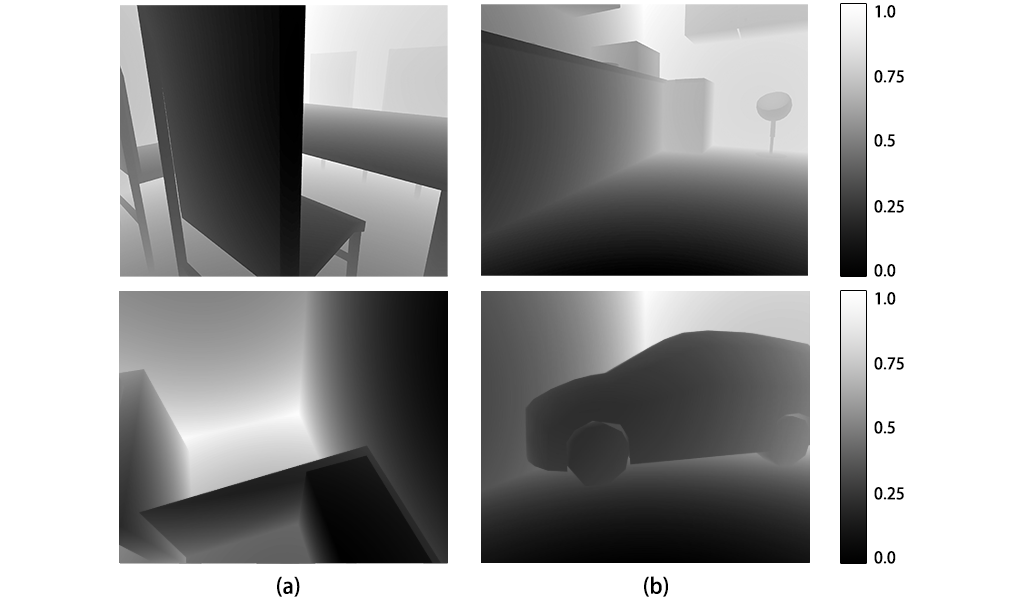
\includegraphics[scale=0.35]{img/depthmap/raw.png}
    \caption{Transient Rendered Scene}
    \label{fig:result_raw}
\end{figure}

We used Nvidia's synthetic data for the initial training of our deep learning model. 
We captured 30 images from different positions of more than 900 different scenes with reflective objects placed in various positions in a room. 
The scenes were first rendered using transient rendering method\cite{jarabo2014} using the same camera FOV as Kinect. 
The noise was then introduced to these scenes using FLAT's Kinect sensor model. 
The model is trained on Kinect data and hence understands the statistical properties of noise from the sensor. 
The model was then retrained on the data that we collected using a Canesta D350 3D Time-of-Flight camera. 
We collected 30 images, each from 20 different scenes. 
All scenes had objects with varied specular properties, thus introducing MPI with the varying amount. 
The ambient light was not controlled, providing very close to real-world conditions.


% -----------------------------------------------------------------------
% Proposed method
% -----------------------------------------------------------------------

\section{Proposed Method}

\begin{figure}
    \centering
    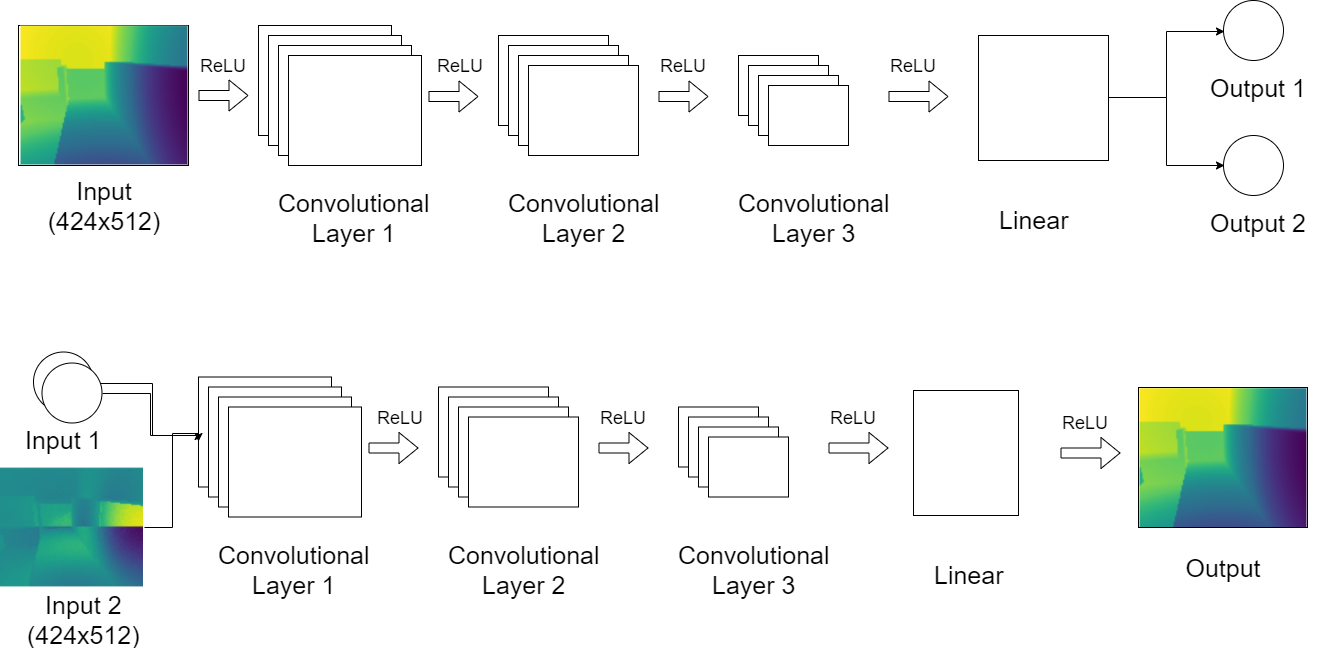
\includegraphics[scale=0.25]{img/NN-model/CNN2.png}
    \caption{Proposed CNN architecture. The first model takes the false depth map of shape (424x512) as input, and outputs the position of camera and specular value of objects in the scene. The second model takes as input the false depth map as well as the output values of first model and provides the accurate depth map as output. }
    \label{fig:result_raw}
\end{figure}

We propose a two-part convolutional neural network model to eliminate MPI noise from images captured using a Time-of-flight camera. 
We demonstrate the use of this model on synthetic data created using the FLAT dataset by Nvidia, which generates Kinect camera-based data. 
\newline
\newline
The first CNN is used to predict scene parameters from a noisy depth map input. 
The ground-truth parameters are available in the synthetic dataset.
The first CNN outputs the correct parameters, which are used as input, along with the noisy depth map, for the second CNN. The input shape of the image is (424x512), and the output values are (4x1) vectors. 
We used three Convolutional layers with a kernel size of 5, a stride value of 1, and a padding value of 2. The output channels were 16, 32, and 64, respectively. 
The convolutional layers were followed by a linear layer that provides vector outputs.
\newline
The second CNN is trained to output the True Depth Map. 
The input to this model is the false depth map image (424x512) and (4x1) parameter vectors. 
The layers of the model have the same hyper-parameters as the first model.
Using such a two-part model gives better control over the training, and provides the model with more information to create accurate depth maps.


% -----------------------------------------------------------------------
% Evaluation
% -----------------------------------------------------------------------

\section{Evaluation}

\begin{figure}
    \centering
    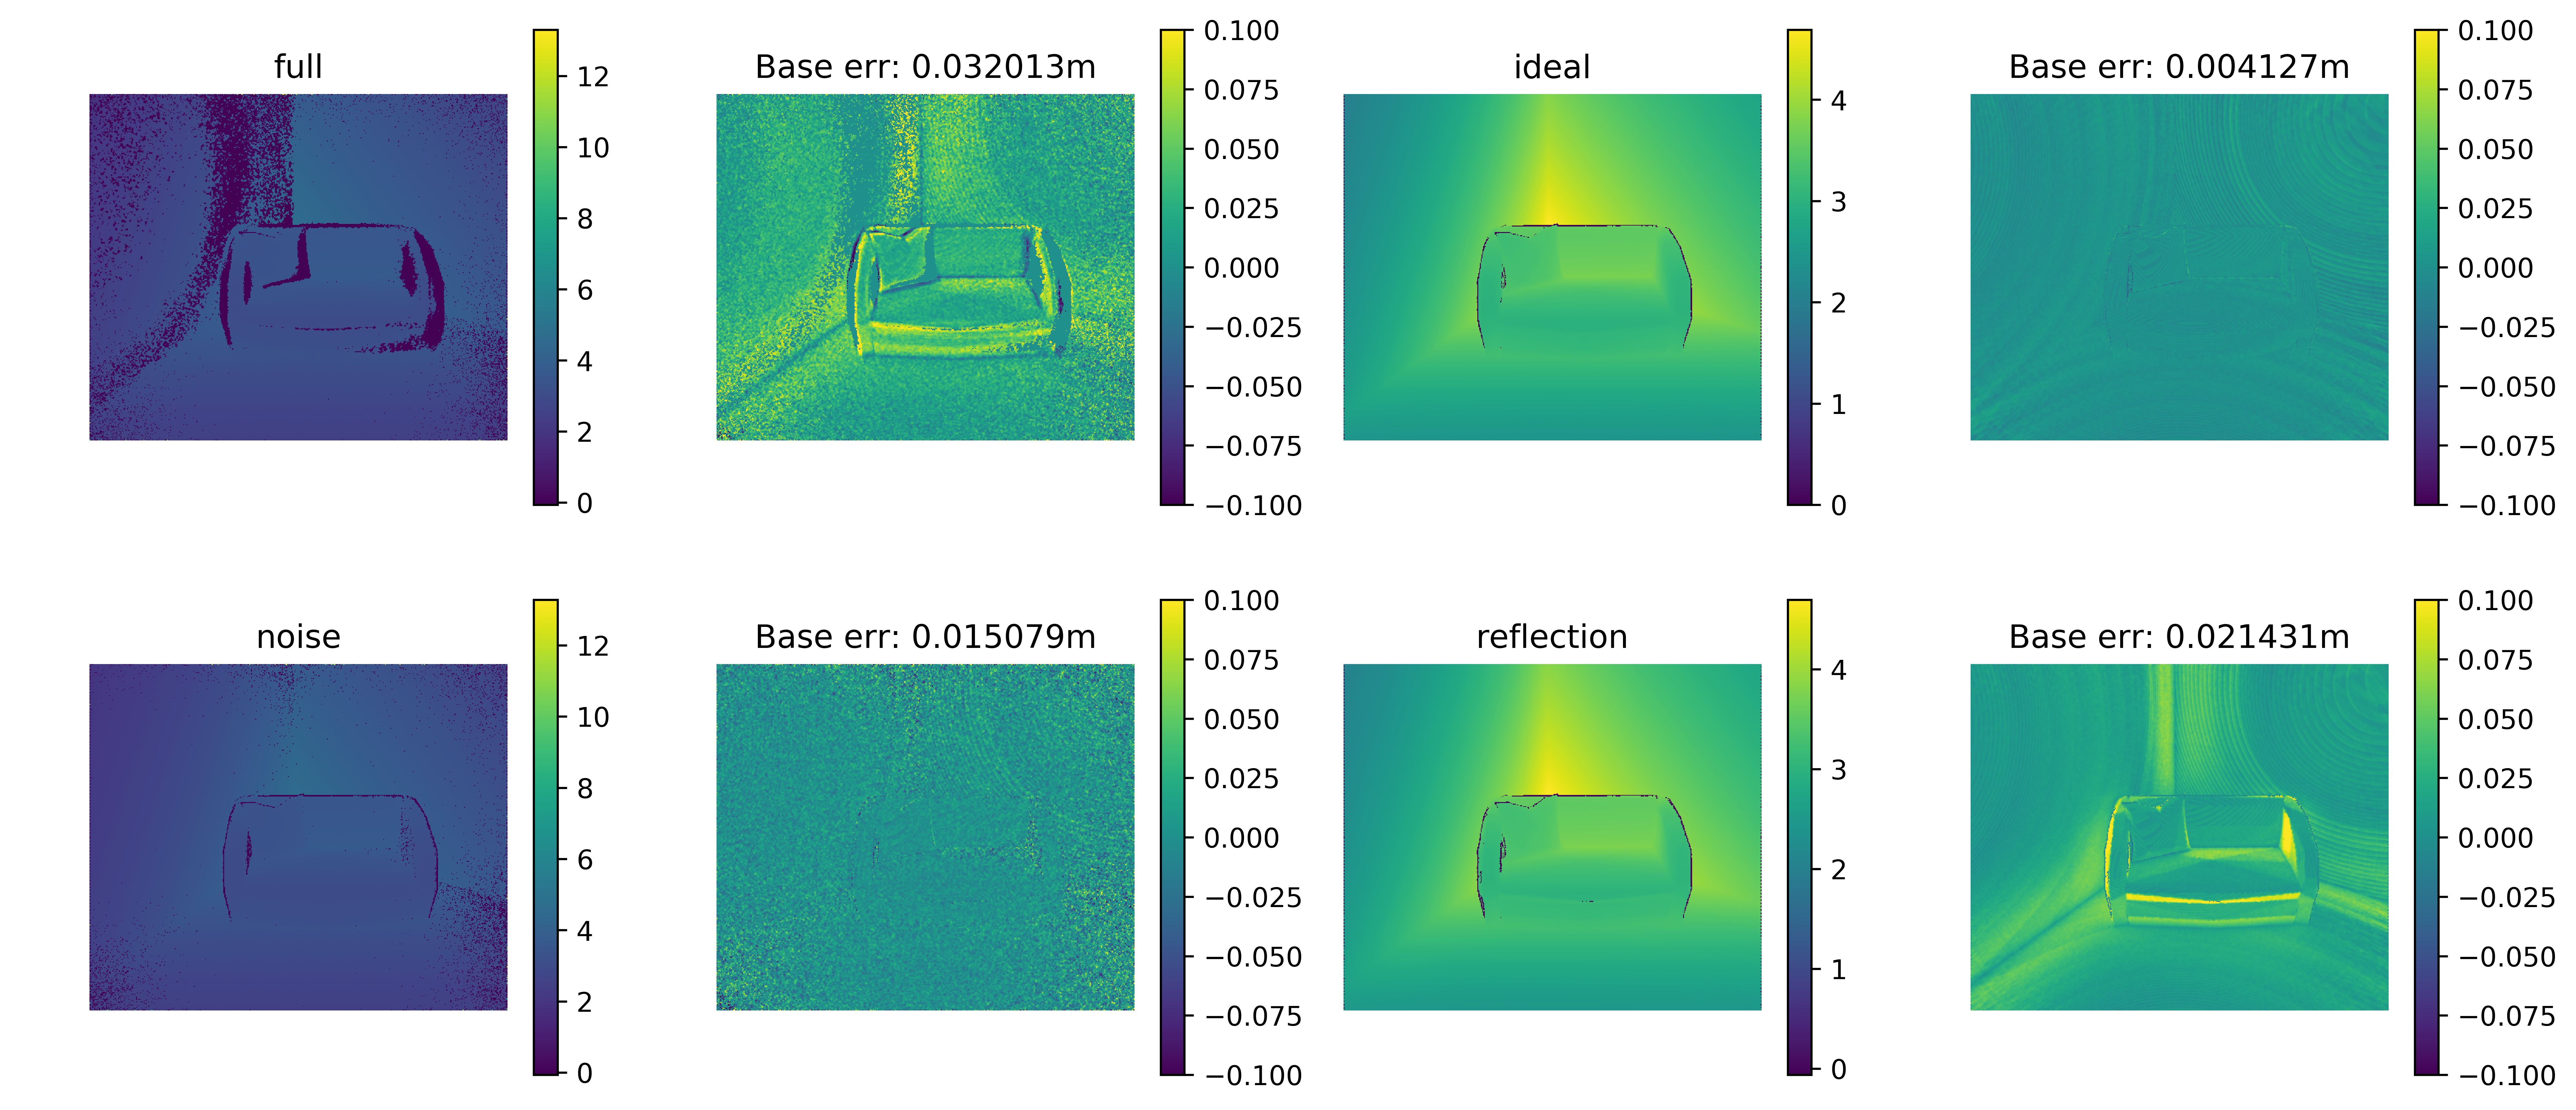
\includegraphics[scale=0.35]{img/depthmap/error.png}
    \caption{Error introduced in ideal images using Kinect mask. Possible noises can be all possible noises(full), sensor noise(noise) and MPI based noise(reflection). }
    \label{fig:result_raw}
\end{figure}

%\lipsum[2-3]
The first model is able to correctly predict the scene parameters to the accuracy of 66.4\%, when the noise (Base Error) present in the data is 0.022050m. 
The second model is able to predict a True Depth Map using the parameters from the first model as input.
\newline
\newline
We evaluated our model's output with respect to NVidia's general pipeline for denoising 3D ToF camera data. 
We also performed comparisons with DeepToF and Phasor. 
We found that our model is able to perform better than Nvidia's Static Multi-Reflection Module (Static MRM). 

% -----------------------------------------------------------------------
% Limitation
% -----------------------------------------------------------------------

\section{Limitations}

The model has been trained on a synthetic dataset. 
The performance on real-dataset is not as good as seen in testing because of the difference in noise statistics between real data and data simulated using the NVidia FLAT simulator. 
Since the model uses noise from the Kinect camera, results for Canesta camera's input depth maps are not of very high accuracy. 
\newline
\newline
We haven't included enough scenes with high specularity, and hence aren't able to handle objects present in a scene with high reflectance such as mirrors or metal surfaces. 

% -----------------------------------------------------------------------
% Conclusion
% -----------------------------------------------------------------------

\section{Conclusions}


Multi-Path Interference based noise is difficult to eliminate because it is difficult to model all possible light paths in a complex scene. 
We have shown a deep learning technique that can be used to remove MPI based noise using a two-part deep learning network. 


% \clearpage\mbox{}Page \thepage\ of the manuscript.
% \clearpage\mbox{}Page \thepage\ of the manuscript.
% \clearpage\mbox{}Page \thepage\ of the manuscript.
% \clearpage\mbox{}Page \thepage\ of the manuscript.
% \clearpage\mbox{}Page \thepage\ of the manuscript.
% \clearpage\mbox{}Page \thepage\ of the manuscript.
% \clearpage\mbox{}Page \thepage\ of the manuscript.
% This is the last page of the manuscript.
% \par\vfill\par
% Now we have reached the maximum size of the ECCV 2018 submission (excluding references).
% References should start immediately after the main text, but can continue on p.15 if needed.

\clearpage

\bibliographystyle{splncs}
\bibliography{egbib}

\appendix
\appendixpage
% \addappheadtotoc

% Temp
\section{Things we had done}


\subsection{Real-world depth data acquisition using Canesta camera}

Using the EP Toolkit, we have successfully managed to captured a set of 100 real-world depth images on various real-world objects, including whiteboards, water bottles, and reflective surfaces, with the Canesta D350 RGB-D Time-of-Flight camera. 
Each image captured is 64 by 64 pixels with RGB values indicating the distance at that pixel.
We have deployed the system on Windows XP Pro (32-bit) running on Oracle VirtualBox in order to run the Toolkit.

\subsection{Setting up the Nautilus Cluster}

Due to the size of the NVlabs FLAT dataset (576GB), we are unable to use the simulator locally on our machines. 
Thus we have successfully deployed the FLAT simulator on the Nautilus Hyper Cluster and using Kubernetes (similar to Docker) for managing the applications. 

Typical Pods in Kubernetes only exist for at most 6 hours, thus it is incapable of performing any training tasks. However, We have managed to migrate the application and the dataset to a persistent storage Pod; this enables us to continue our research and save the progress. We create Jobs and Pods for the purpose of experimenting, training, and evaluating our model on the cloud.


\subsection{Running DeepToF model}

To compare our model with the previous works, we have obtained the trained model from the DeepToF paper. The model was written in Caffe, another hard-to-use deep learning framework. 
We have spent some time researching on how to make the Caffe model run, since it lacks proper documentation. 


\end{document}
